\documentclass[11pt]{article}

\newcommand{\yourname}{Zerun Tian}
\newcommand{\yourcollaborators}{}

\def\comments{0}
\setlength{\parindent}{0 in}
\setlength{\parskip}{0.1in}

%format and packages

%\usepackage{algorithm, algorithmic}
\usepackage[noend]{algpseudocode}
\usepackage{amsmath, amssymb, amsthm}
\usepackage{enumerate}
\usepackage{enumitem}
\usepackage{framed}
\usepackage{verbatim}
\usepackage[margin=1.0in]{geometry}
\usepackage{microtype}
\usepackage{kpfonts}
\usepackage{graphicx}       % upload image
\usepackage{palatino}
	\DeclareMathAlphabet{\mathtt}{OT1}{cmtt}{m}{n}
	\SetMathAlphabet{\mathtt}{bold}{OT1}{cmtt}{bx}{n}
	\DeclareMathAlphabet{\mathsf}{OT1}{cmss}{m}{n}
	\SetMathAlphabet{\mathsf}{bold}{OT1}{cmss}{bx}{n}
	\renewcommand*\ttdefault{cmtt}
	\renewcommand*\sfdefault{cmss}
	\renewcommand{\baselinestretch}{1.06}
\usepackage[usenames,dvipsnames]{xcolor}
\definecolor{DarkGreen}{rgb}{0.15,0.5,0.15}
\definecolor{DarkRed}{rgb}{0.6,0.2,0.2}
\definecolor{DarkBlue}{rgb}{0.2,0.2,0.6}
\definecolor{DarkPurple}{rgb}{0.4,0.2,0.4}
\usepackage[pdftex]{hyperref}
\hypersetup{
	linktocpage=true,
	colorlinks=true,				% false: boxed links; true: colored links
	linkcolor=DarkBlue,		% color of internal links
	citecolor=DarkBlue,	% color of links to bibliography
	urlcolor=DarkBlue,		% color of external links
}

%enclosure macros
\newcommand{\paren}[1]{\ensuremath{\left( {#1} \right)}}
\newcommand{\bracket}[1]{\ensuremath{\left\{ {#1} \right\}}}
\renewcommand{\sb}[1]{\ensuremath{\left[ {#1} \right\]}}
\newcommand{\ab}[1]{\ensuremath{\left\langle {#1} \right\rangle}}

%probability macros
\newcommand{\ex}[2]{{\ifx&#1& \mathbb{E} \else \underset{#1}{\mathbb{E}} \fi \left[#2\right]}}
\newcommand{\pr}[2]{{\ifx&#1& \mathbb{P} \else \underset{#1}{\mathbb{P}} \fi \left[#2\right]}}
\newcommand{\var}[2]{{\ifx&#1& \mathrm{Var} \else \underset{#1}{\mathrm{Var}} \fi \left[#2\right]}}

%useful CS macros
\newcommand{\poly}{\mathrm{poly}}
\newcommand{\polylog}{\mathrm{polylog}}
\newcommand{\zo}{\{0,1\}}
\newcommand{\pmo}{\{\pm1\}}
\newcommand{\getsr}{\gets_{\mbox{\tiny R}}}
\newcommand{\card}[1]{\left| #1 \right|}
\newcommand{\set}[1]{\left\{#1\right\}}
\newcommand{\negl}{\mathrm{negl}}
\newcommand{\eps}{\varepsilon}
\DeclareMathOperator*{\argmin}{arg\,min}
\DeclareMathOperator*{\argmax}{arg\,max}
\newcommand{\eqand}{\qquad \textrm{and} \qquad}
\newcommand{\ind}[1]{\mathbb{I}\{#1\}}
\newcommand{\sslash}{\ensuremath{\mathbin{/\mkern-3mu/}}}

%mathbb
\newcommand{\N}{\mathbb{N}}
\newcommand{\R}{\mathbb{R}}
\newcommand{\Z}{\mathbb{Z}}
%mathcal
\newcommand{\cA}{\mathcal{A}}
\newcommand{\cB}{\mathcal{B}}
\newcommand{\cC}{\mathcal{C}}
\newcommand{\cD}{\mathcal{D}}
\newcommand{\cE}{\mathcal{E}}
\newcommand{\cF}{\mathcal{F}}
\newcommand{\cL}{\mathcal{L}}
\newcommand{\cM}{\mathcal{M}}
\newcommand{\cO}{\mathcal{O}}
\newcommand{\cP}{\mathcal{P}}
\newcommand{\cQ}{\mathcal{Q}}
\newcommand{\cR}{\mathcal{R}}
\newcommand{\cS}{\mathcal{S}}
\newcommand{\cU}{\mathcal{U}}
\newcommand{\cV}{\mathcal{V}}
\newcommand{\cW}{\mathcal{W}}
\newcommand{\cX}{\mathcal{X}}
\newcommand{\cY}{\mathcal{Y}}
\newcommand{\cZ}{\mathcal{Z}}

%theorem macros
\newtheorem{thm}{Theorem}
\newtheorem{lem}[thm]{Lemma}
\newtheorem{fact}[thm]{Fact}
\newtheorem{clm}[thm]{Claim}
\newtheorem{rem}[thm]{Remark}
\newtheorem{coro}[thm]{Corollary}
\newtheorem{prop}[thm]{Proposition}
\newtheorem{conj}[thm]{Conjecture}

\theoremstyle{definition}
\newtheorem{defn}[thm]{Definition}


\newcommand{\instructor}{Virgil Pavlu}
\newcommand{\hwnum}{10}
\newcommand{\hwdue}{Wednesday, May 20 at 11:59pm via \href{https://gradescope.com/courses/229309}{Gradescope}}

\theoremstyle{theorem}
\newtheorem{prob}{}
\newtheorem{sol}{Solution}

\definecolor{cit}{rgb}{0.05,0.2,0.45} 
\newcommand{\solution}{\medskip\noindent{\color{DarkBlue}\textbf{Solution:}}}

\begin{document}
{\Large 
\begin{center}{CS5800: Algorithms} --- Spring '21 --- \instructor \end{center}}
{\large
\vspace{10pt}
\noindent Homework~\hwnum \vspace{2pt}\\
Submit via \href{https://www.gradescope.com/courses/232127}{Gradescope}}

\bigskip
{\large \noindent Name: \yourname }

{\large \noindent Collaborators: \yourcollaborators}

\vspace{15pt}

{\large \noindent Instructions:}

\begin{itemize}

\item Make sure to put your name on the first page.  If you are using the \LaTeX~template we provided, then you can make sure it appears by filling in the \texttt{yourname} command.

\item Please review the grading policy outlined in the course information page.

\item You must also write down with whom you worked on the assignment.  If this changes from problem to problem, then you should write down this information separately with each problem.

\item Problem numbers (like Exercise 3.1-1) are corresponding to CLRS $3^{rd}$ edition.  While the  $2^{nd}$ edition  has  similar  problems  with  similar  numbers,  the  actual  exercises  and their solutions are different, so make sure you are using the $3^{rd}$ edition.

\end{itemize}

%%% Problem 1 %%%
\newpage
\begin{prob} \textbf{(15 points)} Exercise 22.1-5.
\end{prob}
The square of a directed graph $G = (V, E)$ is the graph $G^2 = (V, E^2)$ such that $(u, v) \in E^2$ if and only $G$ contains a path with at most two edges between $u$ and $v$. Describe ... $G^2$ from $G$ for both the adjacency-list and adjacency-matrix of $G$. Analyze the running times of your algorithms.

\solution

For the adjacency-list, we do the following steps to generate $G^2$,
\begin{algorithmic}[1]
\Function{GraphSquaredAdjList}{$G$}
	\State init $G2.\textit{Adj}$ as an array of size $|G.V|$
	\For {$u$ in $G.\textit{Adj}$}
		\State init \textit{added-set} to be an empty set \Comment {to prevent duplicate edges being added to the list}
		\For {$v$ in $G.\textit{Adj}[u]$} \Comment{$(u, v)$ is an edge}
			\State $\textproc{\textsc{ListInsert}}(G2.\textit{Adj}[u], v)$
			\State \textit{added-set}.add($v$)
			\For {$w$ in $G.\textit{Adj}[v]$}	\Comment{$(v, w)$ is an edge, thus $(u, w)$ is a path of 2 edges}
				\If {$w$ not in $\textit{added-set}$}
					\State $\textproc{\textsc{ListInsert}}(G2.\textit{Adj}[u], w)$
				\EndIf
			\EndFor
		\EndFor
	\EndFor
	\State \textbf{return} $G2$
\EndFunction
\end{algorithmic}

For every vertex $u$ in $G.\textit{Adj}$, we scan through every vertex $v$ that is adjacent to $u$. $G2$ will have $(u, v)$ as an edge. Moreover, for every $v$, we find each of its adjacent vertices $w$, which represents an edge $(v, w)$. We know that $(u, w)$ is a path of two edges, which qualifies to belong to $E^2$. We want to avoid adding duplicate vertices in $G2.\textit{Adj}[u]$, so a set data structure called $\textit{added-set}$ is used to take care of this. The for loops at line 5 run at most $O(E)$ iterations, each of which has constant amount of work to do, so the runtime of this algorithm is $O(|V| \cdot |E|)$.

For the adjacency-matrix representation, we do the following steps,
\begin{algorithmic}[1]
\Function{GraphSquaredAdjMatrix}{$A$} \Comment{adjacency matrix $A$ of graph $G$}
	\State $A2 = A \times A$ \Comment {matrix multiplication}
	\For {$i$ in $1$ to $|V|$}
		\For {$j$ in $1$ to $|V|$}
			\If {$A[i, j] == 1$}
				\State $A2[i, j] = 1$
			\EndIf
			\If {$A2[i, j] \ge 1$}
				\State $A2[i, j] = 1$
			\EndIf
		\EndFor
	\EndFor
	\State \textbf{return} $A2$
\EndFunction
\end{algorithmic}

We can easily find paths of two edges by multiplying the matrix $A$ of $G$ by itself. For some index $k$ ($1 \le k \le |V|$), if $(i, k)$ and $(k, j)$ are both 1s' in $A$, it means there is a path of 2 edges between $i$ and $j$ through the vertex $k$. After multiplication, the entry $(i, j)$ in $A2$ will be at least 1 if we can find such $k$s'. To not confuse entry values $\ge 1$ with edge weights, we replace values that are greater than 1 with 1. Furthermore, we copy edges of $G$ into $G^2$ by filling 1 to entry $A2[i, j]$ whenever $A[i, j]$ is 1. The matrix multiplication can be done in $O(|V|^{\lg 7})$ using Strassen’s algorithm shown in book page 82. The for loops take $O(|V|^2)$-time. Overall, the algorithm runs in $O(|V|^{\lg 7}) \approx O(|V|^{2.807})$-time.


%%% Problem 2 %%%
\newpage
\begin{prob} \textbf{(15 points)} Exercise 22.2-6.
\end{prob}

Give an example of a directed graph $G = (V, E)$, a source vertex $s \in V$ , and a set of tree edges $E_{\pi} \subseteq E$ such that for each vertex $v \in V$ , the unique simple path in the graph $(V, E_{\pi})$ from $s$ to $v$ is a shortest path in $G$, yet the set of edges $E_{\pi}$ cannot be produced by running BFS on $G$, no matter how the vertices are ordered in each adjacency list.

\solution

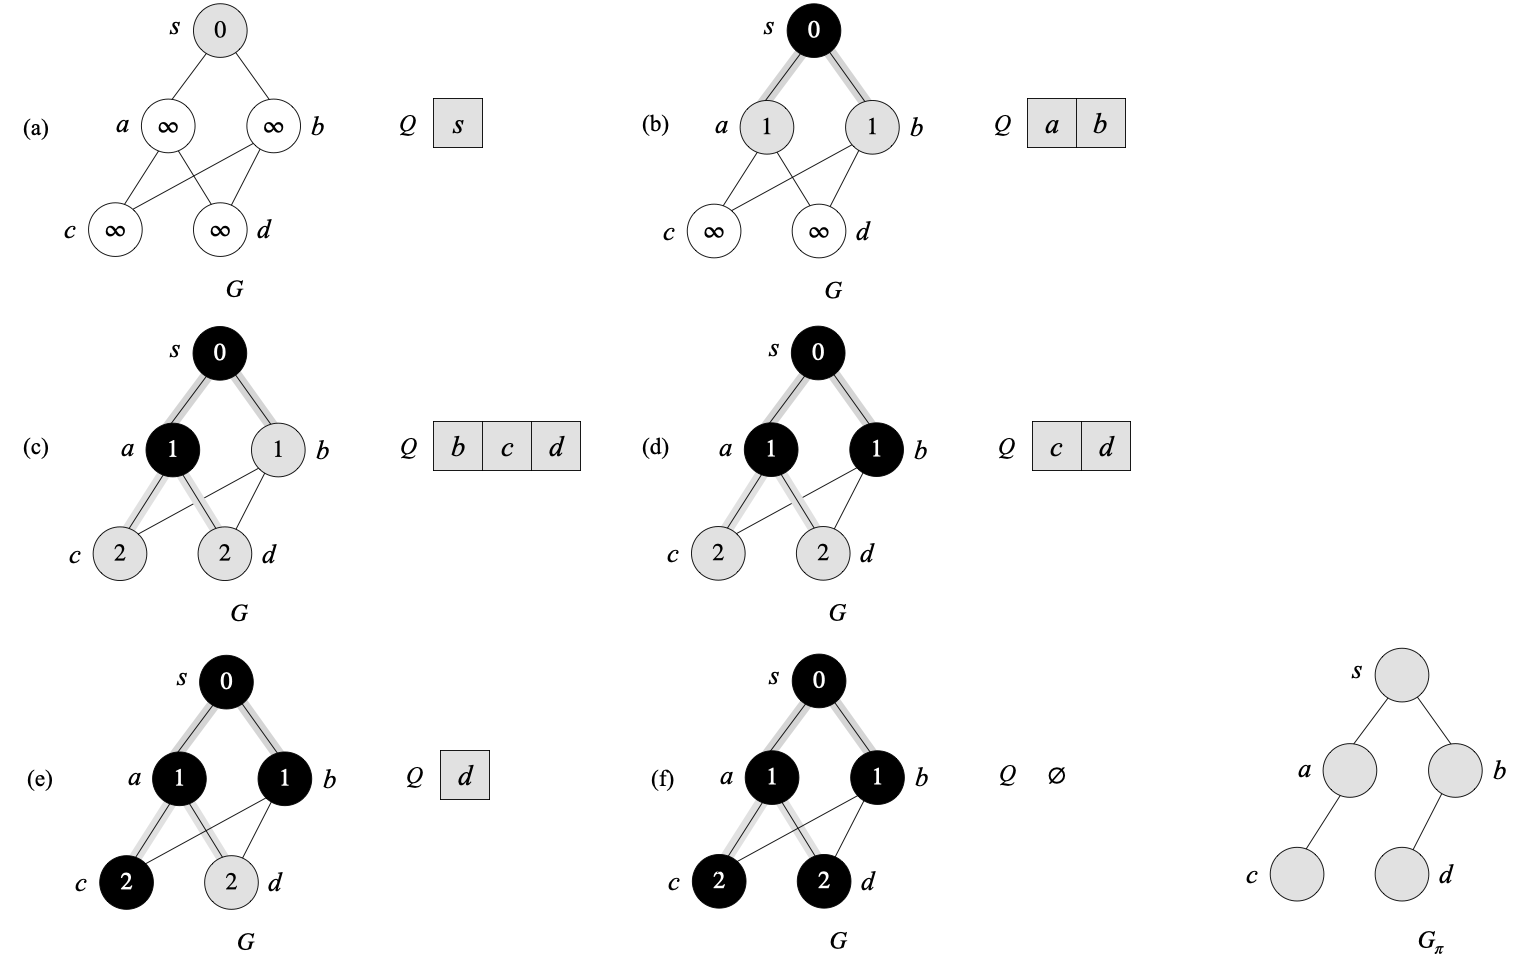
\includegraphics[scale=0.62]{./hw10q2.png}

Diagram (a) shows the graph $G$ with the start vertex added to the $Q$. In (b), we show an example where $a$ appears before $b$ in the adjacency list of vertex $s$. In (c), we pop the vertex $a$ from the $Q$, then we subsequently add its children $c$ and $d$ to the queue (order doesn't matter). It is obvious now that $c$ and $d$'s predecessor is $a$. On the other hand, suppose in (b), we have vertex $b$ appears before $a$ in the adjacency list of vertex $s$. Consequently, the predecessor of $c$ and $d$ will be $b$. In either case, we won't obtain the paths shown in $G_{\pi}$ which yet shows another way we can reach shortest path for every pair of $s$ and $v$.


%%% Problem 3 %%%
\newpage
\begin{prob} \textbf{(15 points)} Exercise 22.2-7.
\end{prob}

There are two types of professional wrestlers: “babyfaces” (“good guys”) and “heels” (“bad guys”). Between any pair of professional wrestlers, there may or may not be a rivalry. Suppose we have $n$ professional wrestlers and we have a list of $r$ pairs of wrestlers for which there are rivalries. Give an $O(n + r)$-time algorithm that determines whether it is possible to designate some of the wrestlers as babyfaces and the remainder as heels such that each rivalry is between a babyface and a heel. If it is possible to perform such a designation, your algorithm should produce it.

\solution

Let's first model this problem as a graph. Each wrestler is a vertex in the graph, and each pair of rivalries is an edge in the graph. We are able to find a designation if the resulting graph exhibits bipartite property which allows us to split vertices into two groups where no edge is present within a group. If so, we can assign one group of vertices to be babyfaces, and the other to be heels, or the other way around. 

To check if the graph is bipartite, we are going to run BFS on a vertex. Meanwhile, we mark vertices with two colors such that vertices of the same wave is colored the same, and vertices of two consecutive waves have alternate colors, say Red and Black. During the process, if we are about to color a vertex that is already colored using a different color from what it currently is, then we conclude that the graph is not a bipartite. After we have run through all vertices and edges, if we did not witness such a case, the graph is a bipartite. Indeed, the graph might not be connected, so we need to run this procedure for all disconnected components of the graph. In the end, we designate all Red vertices as "babyfaces" and the rest as "heels".

In this algorithm, we must go through all edges (rivalries) once. In addition, we visit each vertex at least once yet the total number of visits is upper bounded by number of edges $r$. Thus, the runtime of the algorithm is $O(n + r)$.


%%% Problem 4 %%%
\newpage
\begin{prob} \textbf{(10 points)} Exercise 22.3-7.
\end{prob}

Rewrite the procedure DFS, using a stack to eliminate recursion.

\solution

\begin{algorithmic}[1]
\Function{DFS-Helper}{$G$}
	\State {let $\textit{S}$ be an empty stack}
	\State {\textit{time} = 0}
	\For {each vertex $u \in G.V$}
		\State {$\textit{u.color}$ = \textproc{\textsc{white}}}
		\State {$u.\pi$ = \textproc{\textsc{nil}}}
	\EndFor
	
	\For {each vertex $u \in G.V$} \Comment{in case there are disconnected components}
		\If {$\textit{u.color} == \textproc{\textsc{white}}$} \Comment{the vertex is not yet processed}
			\State {\textit{time} = \textit{time} + 1}
			\State {\textit{u.d} = time} \Comment{$u$ is discovered}
			\State {\textit{u.color} = \textproc{\textsc{gray}}}
                    	\State {$S$.push($u$)} 
                    	\While {$S$ is not empty}
                    		\State {\textit{cur} = $s$.top()} \Comment{peek the top elm without removing it}
				\State {\textit{child} = \textproc{\textsc{nil}}}
                    		\For {each vertex \textit{c} in $G.\textit{Adj}[\textit{cur}]$} \Comment{find the first adjacent vertex that is white}
                    			\If {\textit{c.color} == \textproc{\textsc{white}}}
                    				\State {\textit{child} = c}
						\State \textbf{break}
                    			\EndIf
                    		\EndFor
				\State {\textit{time} = \textit{time} + 1}
				\If {\textit{child} == \textproc{\textsc{nil}}} \Comment {all of cur's adjacency vertices are finished}
					\State {$\textit{cur.f}$ = time} \Comment{$u$ is finished}
					\State {$\textit{cur.color} = \textproc{\textsc{black}}$}
					\State {$S$.pop()} 
				\Else
					\State {$\textit{child}.\pi = \textit{cur}$}
					\State {$\textit{child.d} = \textit{time}$}
					\State {$\textit{child.color} = \textproc{\textsc{gray}} $}
					\State {$S.\textit{push}(\textit{child})$}
				\EndIf
                    	\EndWhile
		\EndIf
	\EndFor
\EndFunction
\end{algorithmic}


%%% Problem 5 %%%
\newpage
\begin{prob} \textbf{(10 points)} Exercise 22.3-10.
\end{prob}

Modify the pseudocode for depth-first search so that it prints out every edge in the directed graph $G$, together with its type. Show what modifications, if any, you need to make if $G$ is undirected.

\solution

We modify the $\textproc{\textsc{DFS-Visit}}$ function such that it prints the edges accordingly, assuming the $\textproc{\textsc{DFS}}$ function shown on page 604 stays as it is

\begin{algorithmic}[1]
\Function{DFS-Visit}{G, u}
	\State {\textit{time} = \textit{time} + 1}
	\State {$u.d = \textit{time}$}
	\State {$\textit{u.color} = \textproc{\textsc{gray}}$}
	\For {each $v \in G.\textit{Adj}[u]$}
		\If {$\textit{v.color} == \textproc{\textsc{white}}$}
			\State \textbf{print} "(" + $u$ + ", " + $v$ + ") is a tree edge"
			\State $v.\pi = u$
			\State \textproc{\textsc{DFS-Visit}}($G$, $v$) 
		\ElsIf {$\textit{v.color} == \textproc{\textsc{gray}}$}
			\State \textbf{print} "(" + $u$ + ", " + $v$ + ") is a back edge"
		\Else  \Comment {$v$ is black}
            		\If {$\textit{u.d} < \textit{v.d}$} \Comment {$u$ is discovered first}
            			\State \textbf{print} "(" + $u$ + ", " + $v$ + ") is a forward edge"
            		\Else
            			\State \textbf{print} "(" + $u$ + ", " + $v$ + ") is a cross edge"
            		\EndIf
		\EndIf
	\EndFor
	\State {$\textit{u.color} = \textproc{\textsc{black}}$}
	\State {\textit{time} = \textit{time} + 1}
	\State {$u.f = \textit{time}$}
\EndFunction
\end{algorithmic}

We don't need to do anything particular for $G$ that is undirected.

%%% Problem 6 %%%
\newpage
\begin{prob} \textbf{(15 points)} Exercise 22.3-12.
\end{prob}

Show that we can use a depth-first search of an undirected graph $G$ to identify the connected components of $G$, and that the depth-first forest contains as many trees as $G$ has connected components. More precisely, show how to modify depth-first search so that it assigns to each vertex $v$ an integer label $\textit{v.cc}$ between 1 and $k$, where $k$ is the number of connected components of $G$, such that $\textit{u.cc} = \textit{v.cc}$ if and only if $u$ and $v$ are in the same connected component.

\solution

It is relatively trivial to identify connected components in an undirected graph. Vertices completely severed from other groups would be considered a separate connected component. We modify the code as follows,

\begin{algorithmic}[1]
\Function{DFS}{G}
	\For {each vertex $u \in G.V$}
		\State {$\textit{u.color}$ = \textproc{\textsc{white}}}
		\State {$u.\pi$ = \textproc{\textsc{nil}}}
	\EndFor
	\State {\textit{time} = 0}
	\State {$k = 1$}
	\For {each vertex $u \in G.V$}
		\If {$\textit{u.color} == \textproc{\textsc{white}}$} \Comment{found an unvisited vertex after the last $\textproc{\textsc{DFS-Visit}}$ if any}
			\State $\textit{u.cc} = k$
			\State \textproc{\textsc{DFS-Visit}}($G$, $u$) \Comment{all vertices reachable from $u$ are explored}
			\State $k = k + 1$
		\EndIf
	\EndFor
\EndFunction
\end{algorithmic}
Notice the line 6, 9, and 11 in the above pseudocode.

$\textproc{\textsc{DFS-Visit}}$ explores all vertices of a connected component given the start vertex $u$. Their labels should be consistent with that of the start vertex $u$.
 
\begin{algorithmic}[1]
\Function{DFS-Visit}{$G$, $u$}
	\State {\textit{time} = \textit{time} + 1}
	\State {$u.d = \textit{time}$}
	\State {$\textit{u.color} = \textproc{\textsc{gray}}$}
	\For {each $v \in G.\textit{Adj}[u]$}
		\If {$\textit{v.color} == \textproc{\textsc{white}}$}
			\State $\textit{v.cc} = \textit{u.cc}$
			\State $v.\pi = u$
			\State \textproc{\textsc{DFS-Visit}}($G$, $v$) 
		\EndIf
	\EndFor
	\State {$\textit{u.color} = \textproc{\textsc{black}}$}
	\State {\textit{time} = \textit{time} + 1}
	\State {$u.f = \textit{time}$}
\EndFunction
\end{algorithmic}

Notice the line 7 in the above pseudocode.


%%% Problem 7 %%%
\newpage
\begin{prob} \textbf{(20 points)} Exercise 22.4-5.
\end{prob}

Another way to perform topological sorting on a directed acyclic graph $G = (V, E)$ is to repeatedly find a vertex of in-degree 0, output it, and remove it and all of its outgoing edges from the graph. Explain how to implement this idea so that it runs in time $O(V + E)$. What happens to this algorithm if $G$ has cycles?

\solution

\begin{algorithmic}[1]
\Function{Typological-Sort}{$G$}
	\State let \textit{indegree} be an array of zeros of size $|G.V|$
	\For {each vertex $u \in G.V$} \Comment {compute in-degree for every vertex}
		\For {each vertex $v \in \textit{G.Adj}[u]$}
			\State $\textit{indegree}[v] = \textit{indegree}[v] + 1$
		\EndFor
	\EndFor
	\State let $Q$ be a queue for storing vertices \Comment{only store vertices of degree 0}
	\For {each vertex $u \in G.V$}
		\If {\textit{indegree}[u] == 0}
			\State $\textit{Q.enqueue}(u)$
		\EndIf
	\EndFor
	\State let \textit{ans} be an empty array to store the sorted vertices
	\While {\textit{Q} is not empty}
		\State $\textit{cur} = \textit{Q.dequeue}()$
		\State $\textit{ans.push}(\textit{cur})$
		\For {each vertex $u \in \textit{G.Adj}[\textit{cur}]$}
			\State $\textit{indegree}[u] = \textit{indegree}[u] - 1$
			\If {$\textit{indegree}[u] == 0$}
				\State $\textit{Q.enqueue}(u)$ 
			\EndIf
		\EndFor
	\EndWhile
	\For {each vertex $u \in G.V$}
		\If {$\textit{indegree}[u] > 0$}
			\State \textbf{error} "failed to do typological sort due to a cycle" \Comment{raises an error}
		\EndIf
	\EndFor
	\State \textbf{return} \textit{ans}
\EndFunction
\end{algorithmic}

From line 2 to 5, we compute the in-degree of every vertex which takes $O(V + E)$-time. From line 6 to 9, we store those vertices of 0 in-degree in a queue. This step takes $O(V)$-time. From line 10 to 17, we iteratively get a vertex with 0 in-degree from the $Q$ and "remove" all its edges by decrementing the in-degree of the respective vertices. This step takes $O(V + E)$-time. After there is no vertex left in the $Q$, we use $O(V)$-time to check if every vertex's in-degree is zero. If so, we can output the vertices in sorted order; otherwise, we claim there is a cycle that refrains us from doing typological sort. Overall, the algorithm runs in $2 \cdot O(V+E) + 2 \cdot O(V)  = O(V + E)$-time.


%%% Problem 8 %%%
\newpage
\begin{prob} \textbf{(15 points)} 
\end{prob}

Two special vertices $s$ and $t$ in the undirected graph G=(V,E) have the following  property:  any  path  from  $s$  to  $t$  has  at  least  $1  +|V|/2$  edges.   Show  that all paths from $s$ to $t$ must have a common vertex $v$ (not equal to either $s$ or $t$) and give an algorithm with running time O(V+E) to find such a node $v$.


\solution

Because there are at least $1 + |V| / 2$ edges from $s$ to $t$, there are at least $1 + |V| / 2$ waves. When there are more than $|V| / 2$ waves, we have to have some waves with only 1 vertex because we don't have enough vertices to put 2 vertices into all waves, and each wave needs to have at least 1 vertex. Therefore, a common vertex $v$ for all paths from $s$ to $t$ can be found in a wave that has only one vertex.

We devise an algorithm that basically modifies $\textproc{\textsc{BFS}}$ to trace such a $v$. Since $\textproc{\textsc{BFS}}$ visits nodes wave by wave, we can maintain a counter to record the number of vertices it has seen in a wave. Specifically, we initialize two variables before the while loop: an integer to count the number of vertices in a wave and a pointer to the previous vertex which $\textproc{\textsc{BFS}}$ visited (dequeued). The counter is initialized as 0, and the pointer is initialized as $\textproc{\textsc{nil}}$. At every iteration of the while loop, we update the counter and pointer accordingly. As soon as we dequeued a vertex whose wave is 1 larger than the current wave, we reset the counter. Before we do the reset, we check if the counter is 1, meaning there is only one vertex present in that wave. We also make sure we are not in the initial wave that contains $s$. If so, a common vertex $v$ is pointed by that pointer we maintained, then we can just return it to caller. In the worst cast, a $v$ is present at the last wave before $t$. The runtime is thus the same as $\textproc{\textsc{BFS}}$, which is $O(V + E)$.


%%% Problem 9 EC %%%
\newpage
\begin{prob} \textbf{(Extra Credit)} Problem 22-3.
\end{prob}
\solution

%%% Problem 10 EC %%%
\begin{prob} \textbf{(Extra Credit)} Problem 22-4.
\end{prob}
\solution


%%% Problem 11 %%%
\newpage
\begin{prob} \textbf{(25 points)} Exercise 23.1-3.
\end{prob}
Show that if an edge $(u, v)$ is contained in some minimum spanning tree, then it is a light edge crossing some cut of the graph.

\solution

Let's remove the edge $(u, v)$ from the minimum spanning tree. Then, we have two minimum spanning trees: one contains the vertex $u$ and the other contains the vertex $v$. Now, we consider a cut that respects the set of edges in both trees and find a cross edge $(u', v')$ that is shorter than $(u, v)$. The $(u', v')$ edge is a safe edge we should pick to construct a minimum spanning tree that does not include $(u, v)$. This makes a contradiction that the $(u, v)$ edge is contained in the minimum spanning tree. Therefore, we proved that the edge $(u, v)$ is indeed a light edge crossing some cut of the graph. 


%%% Problem 12 %%%
\newpage
\begin{prob} \textbf{(25 points)} Exercise 23.2-2.
\end{prob}

Suppose that we represent the graph $G = (V, E)$ as an adjacency matrix. Give a simple implementation of Prim’s algorithm for this case that runs in $O(V^2)$ time.

\solution

\begin{algorithmic}[1]
\Function{MST-Prim-Adj-Matrix}{$G$, $w$, $r$}
	\For {each $u \in G.V$} \Comment {clean up the parent pointer for each vertex}
		\State $u.\pi = \textproc{\textsc{nil}}$
	\EndFor
	\State let $C$ be an array of $\infty$ of size $|G.V|$ \Comment{$C$ stores the min cost to connect the $i$-th vertex to tree}
	\For {$i = 1$ to $|G.V|$} \Comment {update the costs for the root's neighbors}
		\If {$G.A[r, i] == 1$}
			\State $C[i] = w(r, i)$
			\State $i.\pi = r$
		\EndIf
	\EndFor
	\For {$i = 1$ to $|G.V| - 1$}
		\State $\textit{k} = 1$ \Comment {$k$ is the index to the min value of $C$}
		\State $\textit{min-c} = \infty$
		\For {$j = 1$ to $|V|$}
			\If {$C[j] < \textit{min-c}$}
				\State $\textit{min-c} = C[j]$
				\State $k = j$
			\EndIf
		\EndFor
		
		\For {$u = 1$ to $|G.V|$} \Comment {update $k$'s neighbors in $C$}
			\If {$G.A[k, u] == 1$ and $w(k, u) < C[u]$}
				\State $C[u] = w(k, u)$
				\State $u.\pi = k$
			\EndIf
		\EndFor
	\EndFor
\EndFunction
\end{algorithmic}

The algorithm implicitly maintains the minimum spanning tree $A$ of $G$. In the end, we have the tree $A$ as a set of edges that satisfy,
\[
A = \{(v, v.\pi): v \in V - \{r\} \}
\]
It is trivial to see that the for loops of line 2-3, and line 5-8 runs in $O(V)$-time respectively. The for loop of lines 12-15 runs in $O(V)$-time as it iterates through the array $C$ to find the index of the minimum value. The for loop of lines 16-19 has $V$ iterations each of which does constant amount of work. These two loops run in $O(V)$-time within in the for loop at line 9, which results in $O(V \cdot (V-1)) = O(V^2)$-time. Overall, this algorithm runs in $2 \cdot O(V) + O(V^2) = O(V^2)$-time.

%%% Problem 13 %%%
\newpage
\begin{prob} \textbf{(25 points)} Exercise 23.2-4.
\end{prob}

Suppose that all edge weights in a graph are integers in the range from 1 to $|V|$. How fast can you make Kruskal’s algorithm run? What if the edge weights are integers in the range from 1 to $W$ for some constant $W$?

\solution

Because edge weight is in a range of values that is finite and known, we could use counting sort to arrange the edges in non-decreasing order. This pre-kruskal step thus takes $O(E)$ time. The for loop of lines 5-8 in the $\textproc{\textsc{MST-Kruskal}}$ still runs in $O(E \alpha{(V)})$ time per the explantation in page 633 of the book. Overall, the algorithm runs in $O(E) + O(E \alpha{(V)}) = O(E \alpha{(V)})$ time. If the edge weights are integers in the range from 1 to $W$, we still want to use counting sort to speed up the pre-kruskal part to $O(n + k) = O(E + W)$ time. In this case, the algorithm runs in $O(E + W) + O(E \alpha{(V)}) = O(E \alpha{(V)})$ time because $W$ is a constant.


%%% Problem 14 %%%
\newpage
\begin{prob} \textbf{(25 points)} Exercise 23.2-5.
\end{prob}

Suppose that all edge weights in a graph are integers in the range from 1 to $|V|$. How fast can you make Prim’s algorithm run? What if the edge weights are integers in the range from 1 to $W$ for some constant $W$?

\solution

We devise a data structure to replace the queue in the original $\textproc{\textsc{MST-Prim}}$ while keeping the structure of the algorithm. Our goal is to have a new data structure and some auxiliary data to make $\textproc{\textsc{Extract-Min}}$ and $\textproc{\textsc{Decrease-Key}}$ run as fast as possible. 

\begin{algorithmic}[1]
\Function{MST-Prim}{$G$, $w$, $r$}
    \For {each $u \in G.V$}
    	\State $u.\textit{key} = \infty$
	\State $u.\pi = \textproc{\textsc{nil}}$
    \EndFor
    \State let \textit{in-tree} be an empty hash set
    \State let $Q$ be an empty array of size $|V|$
    \State $\textproc{\textsc{AddVertex}}(Q, r, 1)$ \Comment{adding the root vertex to the list at index 1 of the $Q$}
    \State $\textit{np} = \textit{Linkedlist}(1)$ \Comment {$\textit{np}$ maintains indices to non-empty lists of $Q$}
    \While {$Q \ne \emptyset$}
    	\State $u = \textproc{\textsc{Extract-Min}}(Q, \textit{np})$
	\State \textit{in-tree}.add($u$)
	\For {each $v \in \textit{G.Adj}[u]$}
		\If {$v.\textit{key} == \infty$}
			\State $v.\textit{key} = w(u, v)$
			\State $\textproc{\textsc{AddVertex}}(Q, v, w(u ,v))$ \Comment{$O(1)$-time to add a vertex to $Q$}
		\ElsIf {$v \not\in \textit{in-tree}$ and $w(u, v) < \textit{v.key}$}
			\State $v.\pi = u$
			\State $v.\textit{key} = w(u, v)$
			\State $\textproc{\textsc{Decrease-Key}}(Q, v, w(u, v), \textit{np})$ \Comment {move $v$ to the linked list of index $w(u, v)$}
		\EndIf
	\EndFor
    \EndWhile
\EndFunction
\end{algorithmic}

The data structure $Q$ is designed as follows. Let's have an array of size $|V|$ where each element in the array stores a list of vertices that have distance to the prim tree matching the array index. 

To extract a min, we call $\textproc{\textsc{Extract-Min}}(Q, np)$ which finds the first non-empty list in $Q$ through $\textit{np}$ and removes the first node of that list. This is done in $O(1)$ time. The removed node is returned which is added to the prim tree. In addition, for its neighbors whose keys are still $\infty$, we add them to $Q$. Otherwise, for neighbors who are not already in the prime tree, we update their keys and locations in $Q$ to maintain the invariant of our data structure when $w(u, v)$ is indeed smaller than the current $v.\textit{key}$. Thus, $\textproc{\textsc{Decrease-Key}}$ is done in $O(1)$ time to move a node $v$ from where it was to the list at index $w(u, v)$ by just changing several pointers. The $\textproc{\textsc{AddVertex}}$ function is adding a vertex to the list at given index of $Q$, which is done in $O(1)$ time. And notice that, $\textit{np}$, the linked list of indexes to non-empty lists of $Q$, could be managed in $O(1)$-time.

It's trivial to see that the for loop in lines 2-4 runs in $O(V)$ time. Some initializations in lines 5-8 runs in $O(1)$ time. The for loop in lines 12-19 executes $O(E)$ time altogether because the sum of the lengths of all adjacency lists is $2|E|$. Within the for loop, we only have several constant-time operations as detailed earlier. The line 11 and 12 are constant time operations within the while loop at line 9, so $O(V)$ time for that. 

Overall, the algorithm runs in $O(V) + O(1) + O(E) + O(V) = O(E + V)$ time.

Similarly, for integer edge weights in the range from 1 to some constant $W$, we use the same algorithm but initialize $Q$ to be of size $|W|$ to maintain the list of vertices. So, its runtime would also be $O(E + V)$.


%%% Problem 15 EC %%%
\newpage
\begin{prob} \textbf{(Extra Credit)} Problem 23-1.
\end{prob}
\solution

%%% Problem 16 EC %%%
\begin{prob} \textbf{(Extra Credit)} Exercise 23.1-11.
\end{prob}
\solution

%%% Problem 17 EC %%%
\begin{prob} \textbf{(Extra Credit)} Write the code for Kruskal algorithm in a language of your choice. You will first have to read on the disjoint sets datastructures and operations (Chapter21 in the book) for an efficient implementation of Kruskal trees.
\end{prob}
\solution

\end{document}